% set home directory
\providecommand{\homedir}{..} 
% load the preamble of main.tex by subfiles
\documentclass[\homedir/main.tex]{subfiles}
% ##############################################################################
\begin{document}
% set chapter numbering to work correctly even when separate compilation using subfile
\setcounter{chapter}{3}
% ##############################################################################
\chapter{提案手法}\label{chap:methods}
本章では,まず\cref{sec:terms_definition}において提案手法の説明に用いる用語の定義を示す.
次に,\cref{sec:process_flow}で提案手法がデザイン文字列を自動作成する処理の概要を説明する.
その後,\cref{sec:target_design_text}で提案手法が自動作成の対象とするデザイン文字列や,
提案手法の入力として用いる画像が満たすべき条件を明示する.
本章の最後に,\cref{sec:implementation}で\cref{sec:process_flow}で述べた処理の実装について述べる.

% ##############################################################################
\section{用語の定義}\label{sec:terms_definition}
本手法の説明で用いる用語の定義を次の\cref{tab:terms_definition}に示す.

\begin{table}[h]
    \centering
    \caption{用語の定義}
    \begin{tabular}[t]{rl}
        \toprule
        \multicolumn{1}{c}{用語} & \multicolumn{1}{c}{定義}     \\
        \midrule
        コンテンツ                  & 出力されるデザイン文字列で使用したい文字列      \\
        歪みのスタイル                & 出力されるデザイン文字列に付与したい形状の歪み    \\
        エフェクトのスタイル             & 出力されるデザイン文字列に付与したい色やエフェクト  \\
        デザイン文字のグリフ             & デザイン文字に対し,色やエフェクトを無視した文字形状 \\
        \bottomrule
    \end{tabular}
    \label{tab:terms_definition}
\end{table}

また,以下では「バウンディングボックス」を「B.B.」と略記する.
さらに,画像の座標系は左上隅を原点,右向きを$x$軸の正の向き,下向きを$y$軸の正の向きとする.
% ##############################################################################
\section{デザイン文字列の自動作成処理の概要}\label{sec:process_flow}
本手法では,次の\cref{fig:process_flow}のようにしてデザイン文字列を自動作成する.

\begin{figure}[h]
    \centering
    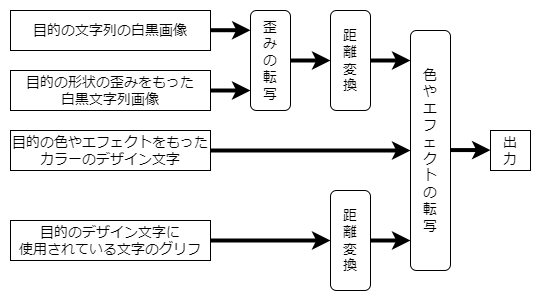
\includegraphics[keepaspectratio, width=0.8\linewidth]{process_flow.png}
    \caption{デザイン文字列の自動作成処理の流れ}
    \label{fig:process_flow}
\end{figure}

\cref{fig:process_flow}に示した処理の流れを順に説明する.

まず,歪みのスタイルを指定する文字列画像からコンテンツを指定する文字列画像へと
文字列の形状の歪みを転写する処理を行う.
この処理は歪みのスタイルを指定する文字列画像の形状の歪みを分析した後,
その歪みを再現するように射影変換を用いてコンテンツを指定する文字列画像を歪ませる
というような手順で実行する.(後の\cref{sec:warp_style_transfer}で詳述する.)

次に,先行研究\cite{typography2019}で提案されたモデルを用いてエフェクトのスタイルを転写するために,
歪みの転写で得た文字列画像と,
エフェクトのスタイルを指定するデザイン文字のグリフを示す画像に対して
距離変換と呼ばれる処理を行う.

最後に,得た二枚の距離変換画像とエフェクトのスタイルを指定するデザイン文字から,
Style Transferを用いて最終的な出力となるデザイン文字列を作成する.
以上が,本手法におけるデザイン文字列の自動作成処理の大まかな流れである.

% ##############################################################################
\section{対象のデザイン文字列}\label{sec:target_design_text}
本手法では,デザイン文字列のうち文字の配置が横一行のもののみを対象とする.
つまり,\cref{sec:background}で述べたようなデザイン文字列に特有のスタイルのうち,
文字列全体の形状の歪みのみを本手法の対象とし,文字の配置や文字の間隔などは対象外とする.

但し,形状の歪みによって文字配置が横一直線でなくなったものも本手法の対象とする.
例えば,次の\cref{fig:warp_and_place}の文字配置は傾いているが,
こうした文字列も本手法の対象とする.

\begin{figure}[h]
    \centering
    
\includegraphics[keepaspectratio, width=0.8\linewidth]{warp_and_place.png}
    \caption{形状の歪みにより,文字配置が傾いた文字列の例}
    \label{fig:warp_and_place}
\end{figure}

さらに,歪みのスタイルの転写元となる画像は次の二つの条件を満たす必要がある.

\begin{enumerate}[label=\textbf{条件\arabic*:}]
    \item 画像中の適切な位置で,
          適切な回数だけ縦に画像を区切ることで左右に画像を分割すれば,
          分割された各領域内の形状の歪みは単純な射影変換で再現できる.
    \item 条件1で述べた適切な画像の分割回数が文字数に比べて十分少ない.
\end{enumerate}

歪みのスタイルの転写元の画像が条件1を満たすとき,
分割された各領域内では,形状の歪みは単純な射影変換で再現できることから,
画像中に含まれる各文字のB.B.の中心の$x$座標に対し,
B.B.の中心の$y$座標とB.B.の大きさがほぼ線形とみなせるといえる.

例えば,次の\cref{fig:poss_warp_wo_guide}は
\cref{fig:poss_warp_with_guide}のように補助線を引くと,
「P」の付近で左半分の領域と右半分の領域の2つの領域に分けることができる.
このとき,左半分の領域の文字列の形状の歪みと右半分の領域のの文字列の形状の歪みは,
どちらも単純な射影変換で再現できるため,
もとの\cref{fig:poss_warp_wo_guide}の画像は条件1を満たすといえる.
\begin{figure}[h]
    \centering
    \begin{minipage}[b]{0.45\linewidth}
        \centering
        
\includegraphics[keepaspectratio, width=0.95\linewidth]{possible_warp_style_without_guide.png}
        \subcaption{もともとの文字列画像}
        \label{fig:poss_warp_wo_guide}
    \end{minipage}
    \begin{minipage}[b]{0.45\linewidth}
        \centering
        
\includegraphics[keepaspectratio, width=0.9\linewidth]{possible_warp_style_with_guide.png}
        \subcaption{補助線を引いた文字列画像}
        \label{fig:poss_warp_with_guide}
    \end{minipage}
    \begin{minipage}[b]{0.45\linewidth}
        \centering
        
\includegraphics[keepaspectratio, width=0.9\linewidth]{possible_warp_style_with_bboxes.png}
        \subcaption{バウンディングボックスつきの文字列画像}
        \label{fig:poss_warp_with_bb}
    \end{minipage}
    \caption{条件1を満たす文字列画像の例}
    \label{fig:possible_warp_style}
\end{figure}
\newpage
一方,\cref{fig:poss_warp_with_guide}と\cref{fig:poss_warp_with_bb}を見比べると,
左半分の領域では右に行くほどB.B.の大きさがほぼ線形に小さくなっており,
右半分の領域では右に行くほどB.B.の大きさがほぼ線形に大きくなっているとわかる.
また,B.B.の中心の$y$座標は\cref{fig:poss_warp_with_bb}を見る限りほぼ一定である.
つまり,この\cref{fig:poss_warp_wo_guide}の画像においては,
画像に含まれる文字のB.B.の中心の$x$座標に対し,
B.B.の中心の$y$座標とB.B.の大きさが区分的にほぼ線形であるといえる.

この例からは,歪みのスタイルの転写元の画像が条件1を満たすとき,
画像に含まれる文字のB.B.の中心の$x$座標に対し,
B.B.の中心の$y$座標とB.B.の大きさが区分的にほぼ線形となり,
区間の境界と形状の歪み方が切り替わる位置がほぼ一致することが予想できる.

この予想が正しいと仮定すると,
歪みのスタイルの転写元の画像として\cref{fig:poss_warp_wo_guide}のような画像が与えられたとき,
\cref{fig:poss_warp_with_bb}のように各文字のB.B.を計算した後に,
得たB.B.の中心の$x$座標に対し,B.B.の中心の$y$座標とB.B.の大きさを区分線形回帰することで,
区間の境界位置として形状の歪みの切り替わる位置を推定し,
\cref{fig:poss_warp_with_guide}のような形状の歪みの情報を計算することができる.
これが歪みのスタイルの転写元の画像が条件1を満たすべき理由である.

また,歪みのスタイルの転写元の画像が条件2を満たすとき,
分割された各領域内には十分多くの文字が含まれることになる.
これは上述したように区分線形回帰を用いて形状の歪みの切り替わる位置を推定する際に,
回帰の精度を保証するために必要な条件であるため,
歪みのスタイルの転写元の画像は条件2も満たすべきである.

%TODO 扱えるもの,扱えないものの具体例の図を増やす
%本節の最後に,扱える文字列の歪みと扱えない文字列の歪みについて具体例をいくつか示す.~

% ##############################################################################
\section{実装}\label{sec:implementation}
\subsection{歪みのスタイルの転写}\label{sec:warp_style_transfer}
歪みのスタイルの転写処理は\cref{sec:process_flow}で簡単に述べたように,
歪みのスタイルの転写元の画像を分析して目的とする歪みのスタイルの情報を得る処理と,
得た情報を元に歪みのスタイルの転写先の画像を射影変換を用いて歪ませる処理の,
二つに大きく分けられる.

このうち,歪みのスタイルの情報を得る処理は,
\cref{sec:target_design_text}で歪みのスタイルの転写元の画像が
2つの条件を満たすべき理由として述べたように区分線形回帰を用いて実行する.

但し,\cref{sec:target_design_text}では
分割された領域内の形状の歪みが同じになるように領域を分割するとき,
分割後の領域数として最適な値の決定方法については考慮していなかった.
そのため,実際に歪みのスタイルの転写元の画像のみから
歪みのスタイルの情報を得る際には,
分割後の領域数として最適な値を自動的に決定できるように
アルゴリズムを修正しなければならない.

そして,修正したアルゴリズムの疑似コードが次の\cref{alg:warp_style_transfer}である.
このアルゴリズムでは,
分割後の領域数を1から初めて徐々に増やしながら繰り返し区分線形回帰を実行していく.
そして,回帰の二乗平均平方根誤差が閾値以下となるか,
ひとつ前のループの回帰の二乗平均平方根誤差との差分が閾値以上であった場合,
そのループにおける区分線形回帰の結果を採用して計算を終了する.
逆に,ひとつ前のループに比べて二乗平均平方根誤差が悪化した場合は,
ひとつ前のループの区分線形回帰の結果を採用して計算を終了する.
また,分割後の領域数が画像の文字数の半分を上回った場合は計算を強制終了し,
最後のループにおける区分線形回帰の結果を採用する.
なお,区分線形回帰の実装にはpythonのライブラリであるpiecewise linear fittingを用いた.
以上のようにして得た歪みのスタイルの情報を元に,
スタイルの転写先の画像を射影変換を用いて歪ませることで歪みのスタイルを転写する.
なお,射影変換の実装にはpythonのライブラリであるOpenCV を用いた.

\begin{algorithm}[h]
    \caption{歪みのスタイルの情報の推定}
    \label{alg:warp_style_transfer}
    \begin{algorithmic}[1]
        \Require{
            \Statex $warped\_image$:歪みのスタイルを指定する白黒画像
            \Statex $\varDelta~\varepsilon$:区分線形回帰の二乗平均平方根誤差の差分の閾値
            \Statex $\varepsilon$: 区分線形回帰の二乗平均平方根誤差の閾値
        }
        \Ensure{
            \Statex $fit\_result$:区分線形回帰の結果
        }
        \Function {transfer\_warp\_style}{$target\_image, warped\_image, \varDelta~\varepsilon, \varepsilon$}
        \State $bounding\_boxes$ = \Call{GET\_BOUNDING\_BOXES}{$warped\_image$}
        \State $num\_boxes$ = \Call{GET\_LENGTH}{$bounding\_boxes$}

        \State $num\_segments$ = 1
        \While{$num\_segments \leq num\_boxes/2$}
        \State $fit\_result$ = \Call{PIECEWISE\_LINEAR\_FIT}{$bounding\_boxes, num\_segments$}
        \State $error$ = \Call{GET\_FITTING\_ERROR}{$fit\_result$}

        \If{$num\_segments \neq 1$}
        \If{$prev\_error - error < 0$}
        \State $fit\_result = prev\_fit\_result$
        \State \Break
        \ElsIf{$prev\_error - error > \varDelta~\varepsilon$ \OR $error \leq \varepsilon$}
        \State \Break
        \EndIf
        \EndIf
        \State $num\_segments = num\_segments + 1$
        \State $prev\_fit\_result$ = $fit\_result$
        \State $prev\_error$ = $error$

        \EndWhile
        \State \Return $fit\_result$
        \EndFunction

    \end{algorithmic}
\end{algorithm}

\subsection{距離変換およびエフェクトのスタイルの転写}
エフェクトのスタイルの転写処理は\cref{sec:process_flow}で簡単に述べたが,
先行研究\cite{typography2019}で提案されたモデルを用いて実行する.



% ##############################################################################
\printBibForSubfiles
\end{document}